% !TEX root = ../main.tex
\subsubsection{Electron Variables}
\label{14.21::electron_variables}
    The acceptance of the scattered electron variables $Q^2$ and $\nu$ is presented in Figure \ref{fig::14.21::electron_acc}.
    Each one is shown in an integrated kinematical region for the other variable.

    \begin{figure}[t!]
        \centering
        % Q2.
        \begin{subfigure}[b]{\textwidth}
            \centering
            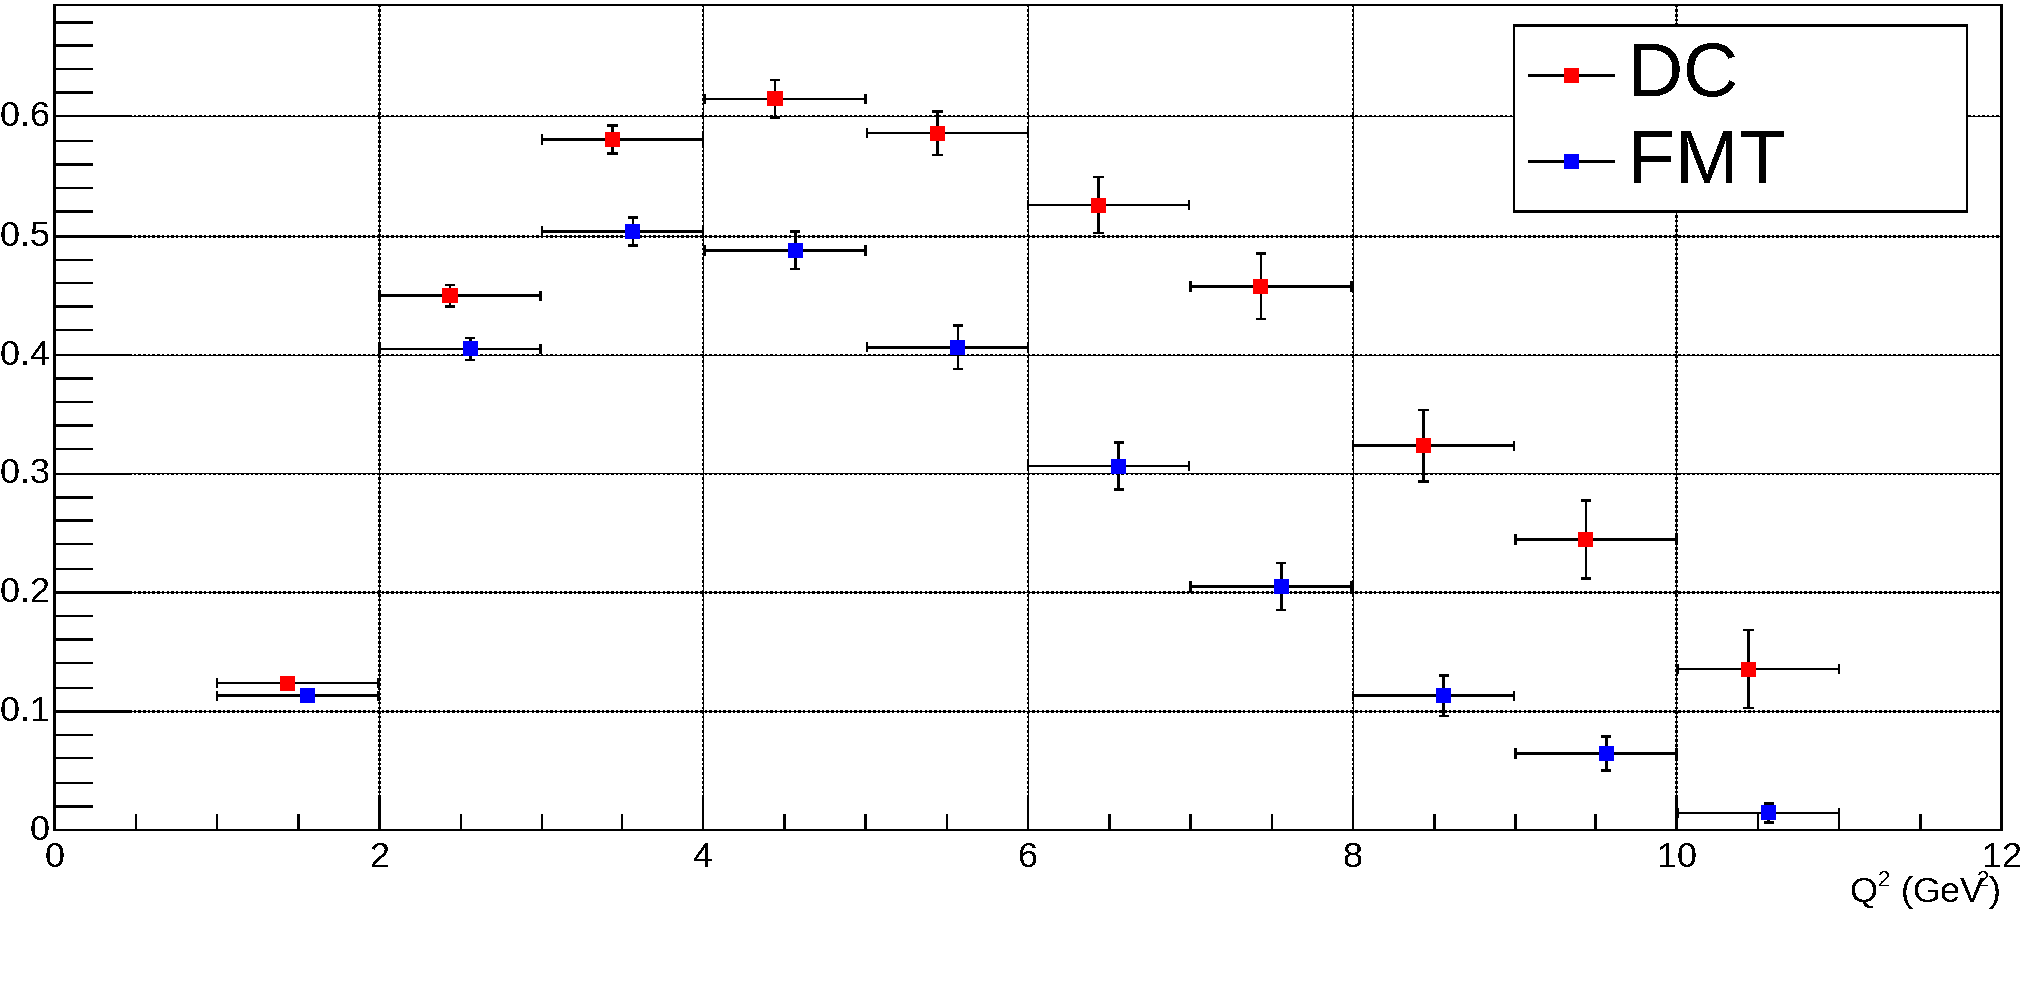
\includegraphics[width=\textwidth]{21q2_acc.pdf}
            \caption{$Q^2$ acceptance.}
            \label{fig::14.21::q2_acc}
        \end{subfigure}
        \hfill
        % nu.
        \begin{subfigure}[b]{\textwidth}
            \centering
            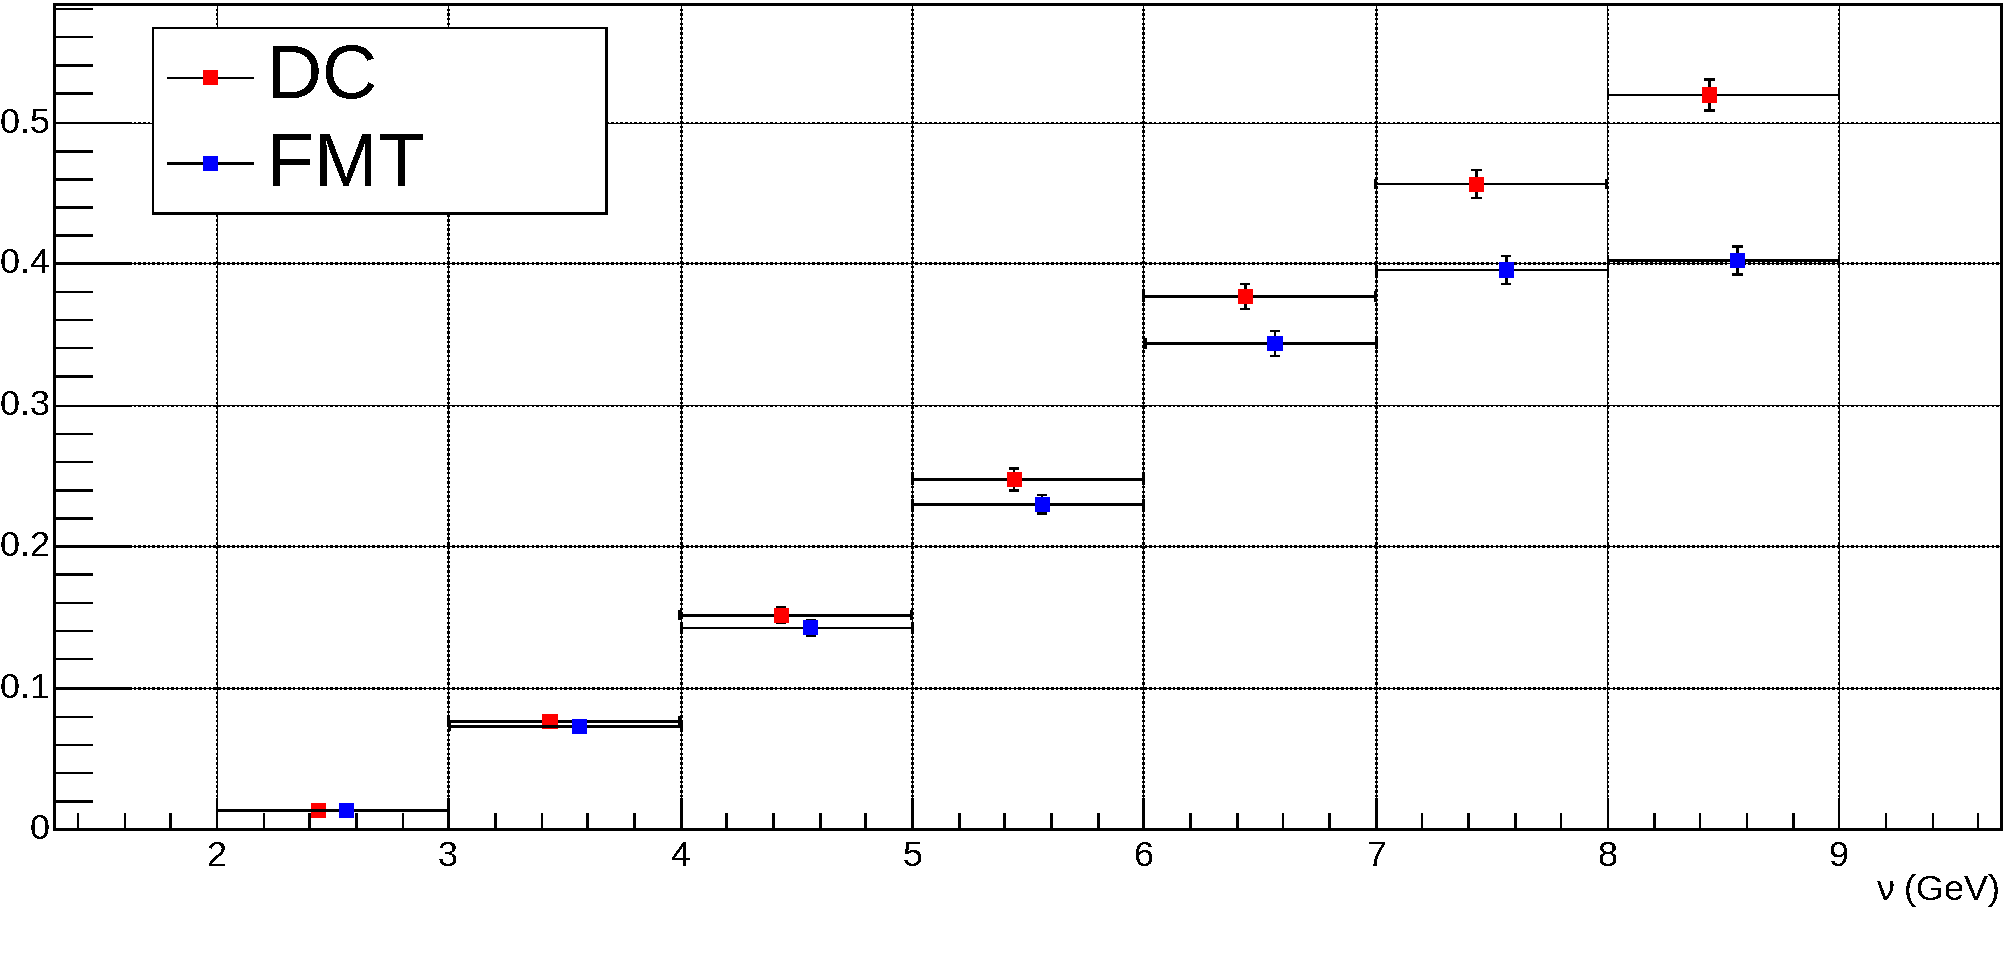
\includegraphics[width=\textwidth]{21nu_acc.pdf}
            \caption{$\nu$ acceptance.}
            \label{fig::14.21::nu_acc}
        \end{subfigure}
        \caption[$e^-$ variables acceptance]
        {$e^-$ variables acceptance.
        $\nu$ is integrated in \ref{fig::14.21::q2_acc}, and $Q^2$ is integrated in \ref{fig::14.21::nu_acc}.
        The bin markers are slightly shifted in $x$ to improve legibility.}
        \floatfoot{Source: Own elaboration, using the \href{https://github.com/bleaktwig/clas12-rge-analysis}{clas12-rge-analysis} software.}
        \label{fig::14.21::electron_acc}
    \end{figure}

    \begin{figure}
        \centering
        % phi vs. theta.
        \begin{subfigure}[b]{\textwidth}
            \centering
            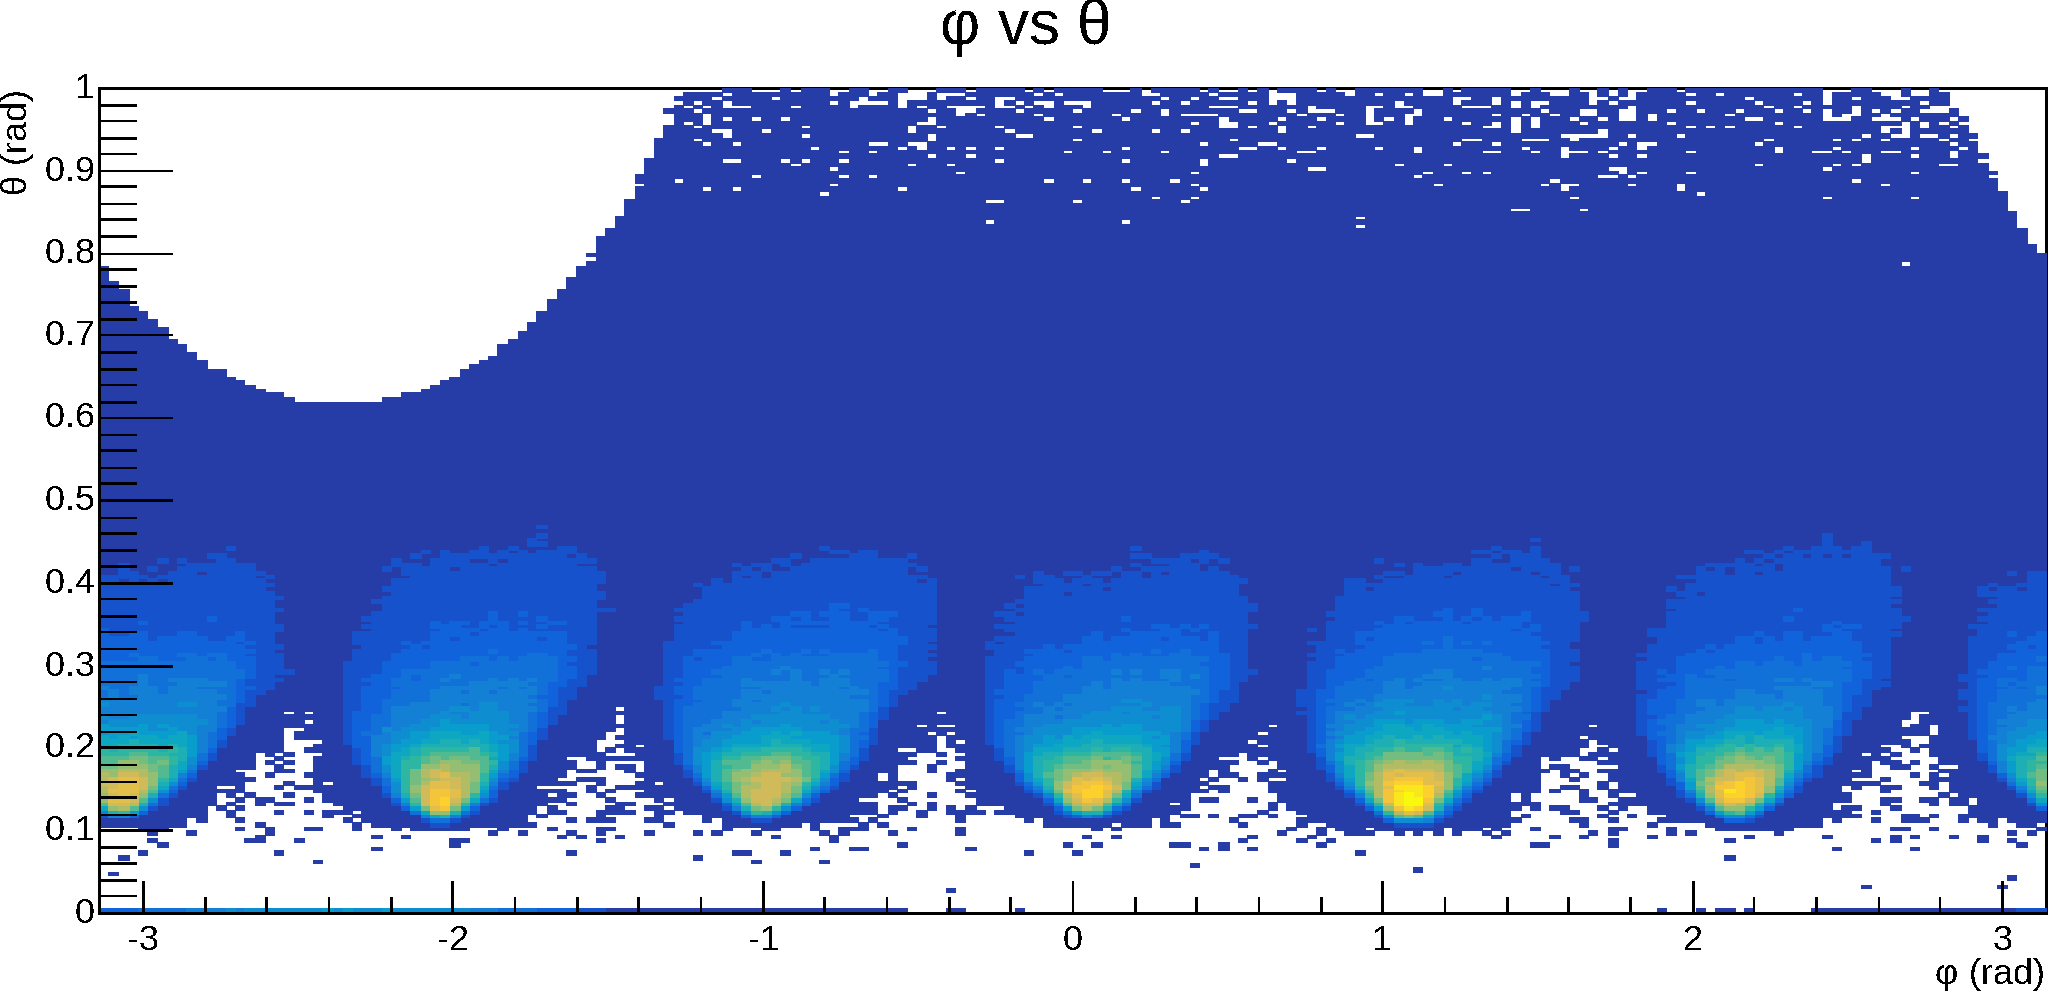
\includegraphics[width=\textwidth]{21phi_theta_neg.pdf}
            \caption[$\phi$ vs. $\theta$ for negative particles]
            {$\phi$ vs. $\theta$ for negative particles detected by DC.
            The sector with less acceptance than the rest is caused by \textbf{TODO}.}
            \label{fig::14.21::phi_theta_neg}
        \end{subfigure}
        % theta.
        \begin{subfigure}[b]{\textwidth}
            \centering
            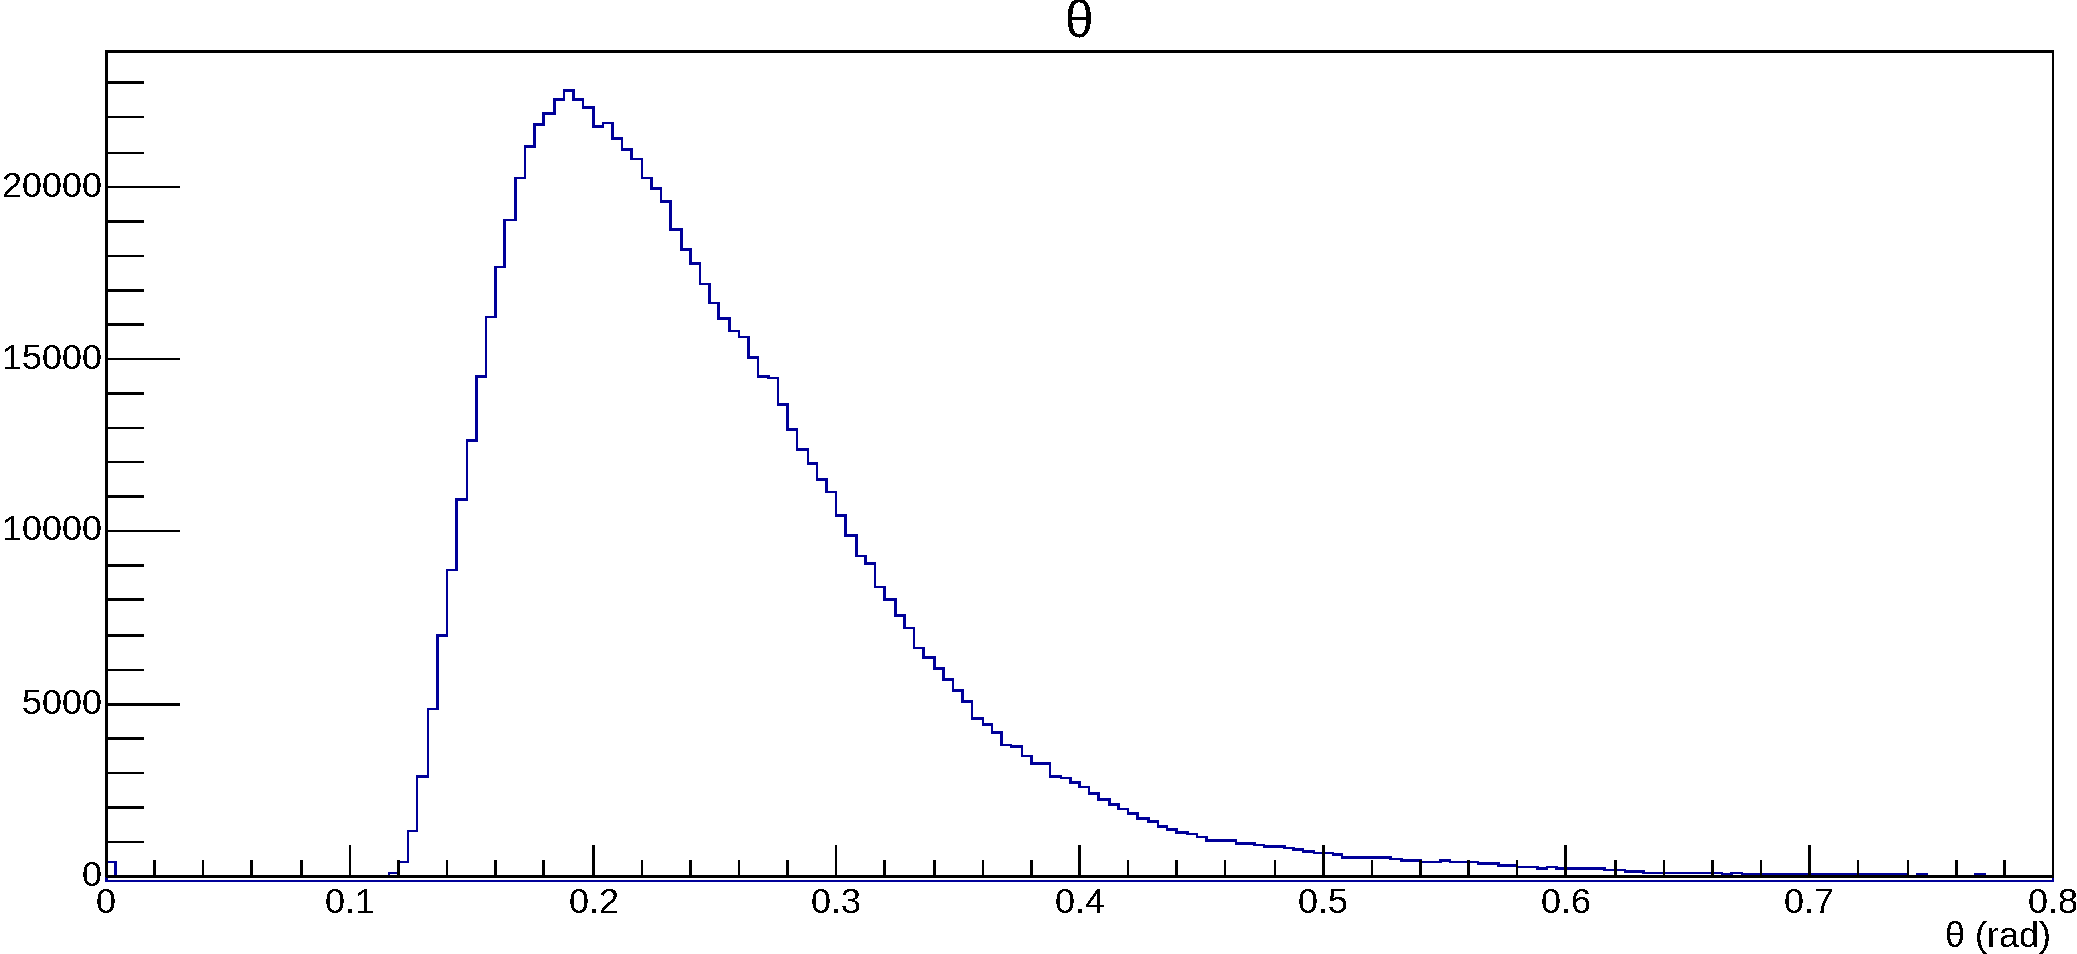
\includegraphics[width=\textwidth]{21theta_neg.pdf}
            \caption[$\theta$ for negative particles]
            {$\theta$ for negative particles detected by DC.}
            \label{fig::14.21::theta_neg}
        \end{subfigure}
        \caption[$\theta$ study for negative particles]
        {$\theta$ study for negative particles.
        Simulated RG-F target.}
        \floatfoot{Source: Own elaboration, using the \href{https://github.com/bleaktwig/clas12-rge-analysis}{clas12-rge-analysis} software.}
        \label{fig::14.21::theta_study_neg}
    \end{figure}

    % Q2.
    In Equation \eqref{eq::13.23::q2}, it can be observed that $Q^2$ has a quadratic dependence on the scattering angle $\theta_C$ of the scattered electrons.%, particularly for small angles.
    Hence, it is important to understand the $\theta$ acceptance of CLAS12 in order to distinguish the geometric effect related to $\theta$ from the inherent $Q^2$ acceptance of the FD.
    Figure \ref{fig::14.21::theta_study_neg} illustrates this dependence for negative particles.

    The triangular shape of each DC sector, combined with the inbending tracks resulting from the negative solenoid field, leads to a significantly low acceptance at low $\theta$ angles.
    When integrating across $\phi$, this results in a low $\theta$ efficiency for $\theta \lsim 0.15$ radians.
    Referring back to the $Q^2$ plot in Figure \ref{fig::14.21::q2_acc}, the decrease in $Q^2$ acceptance between 1 and 4 $GeV^2$ can be clearly attributed to this geometric effect, which is purely of a geometric nature.

    % nu
    On the other hand, since $\nu$ does not exhibit a direct correlation with $\theta_C$ (as indicated by Equation \eqref{eq::13.23::nu}), we can assume that the acceptance observed in Figure \ref{fig::14.21::nu_acc} is intrinsic to the detector.
